
% !TeX root = ../../main.tex
\subsection{Envio e Recebimento de dados via Iperf3}


Para esta simulação, foi realizada a transmissão de um arquivo FTP e de um arquivo de voz. Para 
isso foi utilizada a ferramenta Iperf3, com o Host Zabbix atuando como servidor e o Host Snort como cliente. 
O teste de largura de banda entre os hosts foi realizado utilizando o protocolo TCP.

Na primeira simulação, foi realizada a transmissão de um arquivo FTP do Host Snort para o Host Zabbix. Na Figura \ref{fig:iperf2},
 é possível observar o comando utilizado para iniciar o servidor Iperf3 no Host Zabbix, 
 bem como o resultado do teste de largura de banda entre os dois hosts. 
 O teste indicou uma largura de banda de 1 Gbps,
  demonstrando a capacidade da rede para suportar a transferência de arquivos FTP de forma eficiente.


\begin{figure}[H]
    \centering
    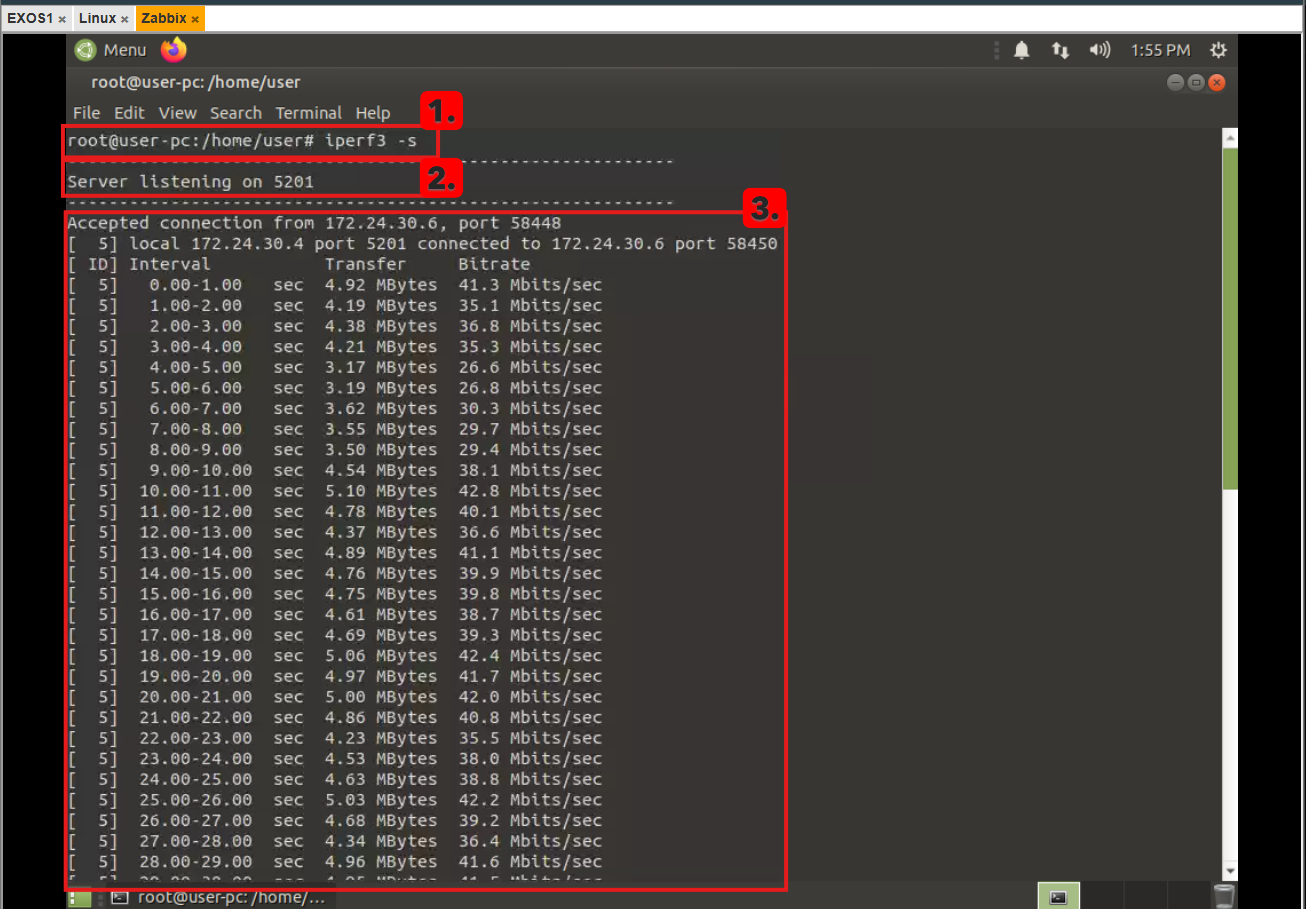
\includegraphics[width=1\linewidth]{fig/iperf/iperf2.png}
    \caption{Host Zabbix como servidor Iperf3 - transmissão arquivo FTP; 1. Comando para iniciar o servidor Iperf3; 
    2. Resultado do teste de largura de banda entre o Host Zabbix e o Host Cliente}
    \label{fig:iperf2}
\end{figure}

Na Figura \ref{fig:iperf1}, é possível observar o comando, \textit{iperf3 -c 172.24.30.10 -i 10 -p 5201 -w 8.0K -t 60},
utilizado para iniciar o cliente Iperf3 no Host Snort. O \textit{-c} especifica o endereço IP do servidor, 
\textit{-i} define o intervalo de tempo para exibir os resultados, 
\textit{-p} indica a porta utilizada para a comunicação, 
\textit{-w} define o tamanho da janela TCP e 
\textit{-t} especifica a duração do teste em segundos.

  
Ainda na Figura \ref{fig:iperf1}, é possível ver o resultado do teste de largura de banda entre o Host Snort e o Host Zabbix. 
O teste indicou uma largura de banda de 1 Gbps, confirmando a capacidade da rede para suportar a
transferência de arquivos FTP de forma eficiente.

\begin{figure}[H]
    \centering
    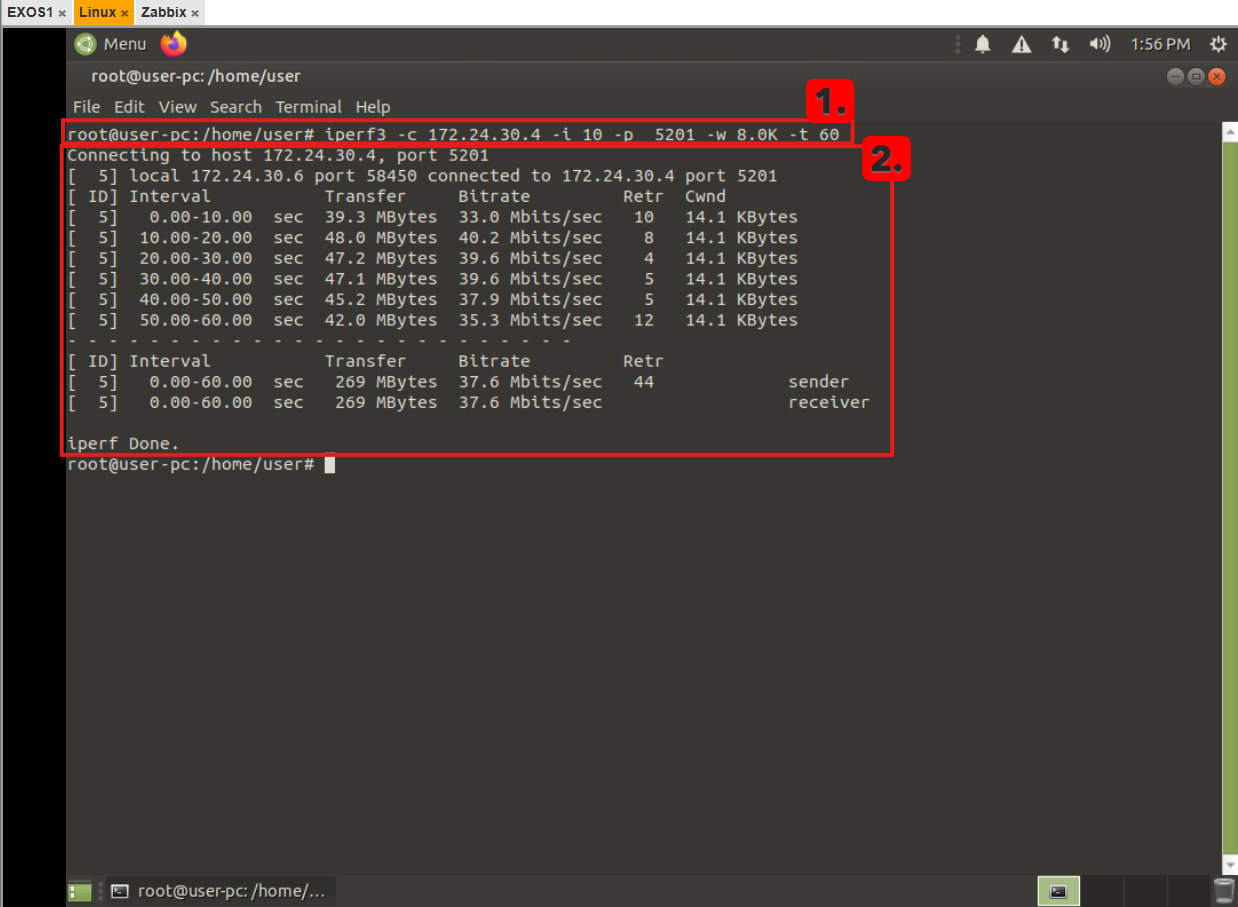
\includegraphics[width=1\linewidth]{fig/iperf/iperf1.png}
    \caption{Host Snort como cliente Iperf3 - transmissão arquivo FTP; 1. Comando para iniciar o cliente Iperf3; 
    2. Resultado do teste de largura de banda entre o Host Snort e o Host Zabbix}
    \label{fig:iperf1}
\end{figure}

Já na segunda simulação, foi realizada a transmissão de um arquivo de voz do Host Snort para o Host Zabbix.
Na Figura \ref{fig:iperf3}, é possível observar o comando utilizado para iniciar o servidor Iperf3 no Host Zabbix,
bem como o resultado do teste de largura de banda entre os dois hosts.

\begin{figure}[H]
    \centering
    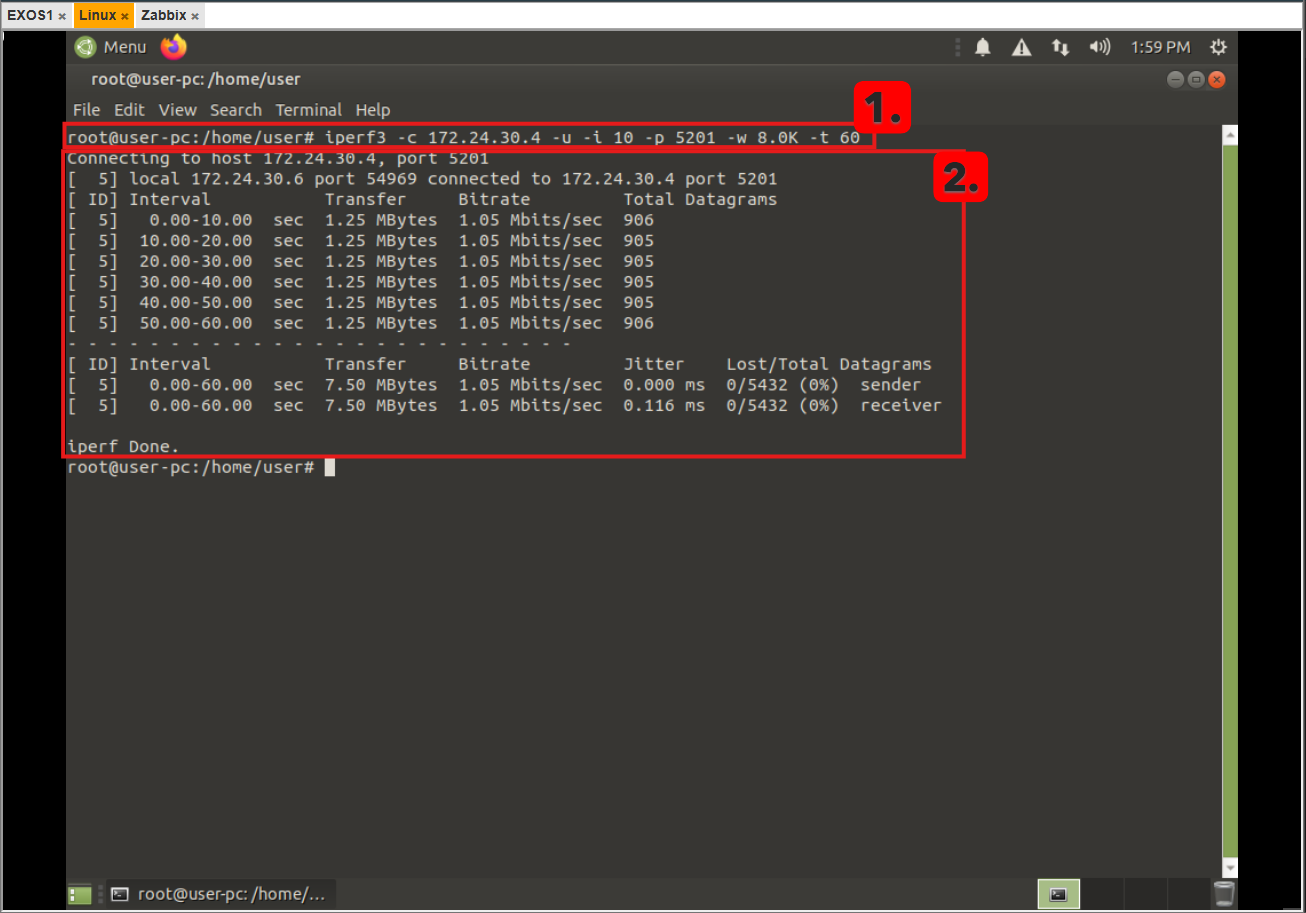
\includegraphics[width=1\linewidth]{fig/iperf/iperf3.png}
    \caption{Host Zabbix como servidor Iperf3 - transmissão arquivo de Voz; 1. Comando para iniciar o servidor Iperf3; 
    2. Resultado do teste de largura de banda entre o Host Zabbix e o Host Cliente}
    \label{fig:iperf3}
\end{figure}

Na Figura \ref{fig:iperf4}, é possível observar o comando,\textit{iperf3 -c 172.24.30.10 -u -i 10 -p 5201 -w 8.0K -t 60},
utilizado para iniciar o cliente Iperf3 no Host Snort. No comando, o \textit{-c} especifica o endereço IP do servidor,
O \textit{-u} especifica que o teste deve ser realizado utilizando o protocolo UDP, 
\textit{-i} define o intervalo de tempo para exibir os resultados,
\textit{-p} indica a porta utilizada para a comunicação, 
\textit{-w} define o tamanho da janela TCP e \textit{-t} especifica a duração do teste em segundos.    

Ainda na Figura \ref{fig:iperf4}, é possível ver o resultado do teste de largura de banda entre os dois hosts. O teste indicou uma largura de banda de 1 Gbps,
 demonstrando a capacidade da rede para suportar a transferência de arquivos de voz de forma eficiente.

\begin{figure}[H]
    \centering
    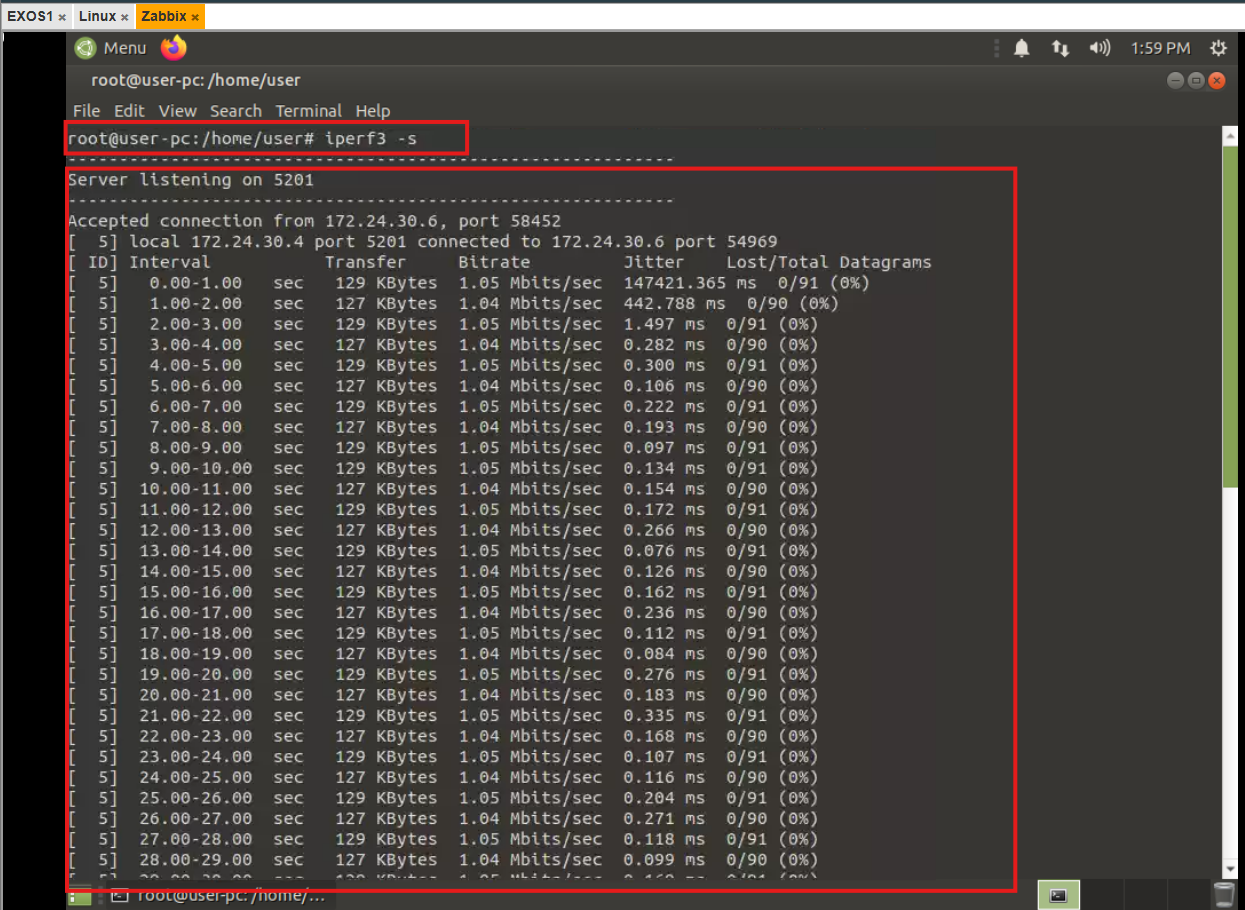
\includegraphics[width=1\linewidth]{fig/iperf/iperf4.png}
    \caption{Host Snort como cliente Iperf3 - transmissão arquivo de Voz; 1. Comando para iniciar o cliente Iperf3; 
    2. Resultado do teste de largura de banda entre o Host Snort e o Host Zabbix}
    \label{fig:iperf4}
\end{figure}